  
\section{Properties of the chords and variation of length}

In this section we obtain some  properties of chords of convex curves and applications in billiard orbits.
 
Consider two regular convex curves $\gamma$ and $\Gamma$ parametrized by arc lengths $s$ and $t$. 
Let $l(s,t)=|\gamma(s)-\Gamma(t)|$, $\theta(s,t) $ the angle between $\gamma^\prime(s)$ and $V(s,t)=\Gamma(t)-\gamma(s)$ and  $\eta(s,t) $ the angle between $\Gamma^\prime(t)$ and $V(s,t)$. See Fig. \ref{fig:1corda}

Consider the Frenet frames $\{\gamma^\prime (s), N_\gamma\}$ and $\{\Gamma^\prime (t), N_\Gamma\}$ along $\gamma$ and $\Gamma$.  Denote the curvatures by $k_\gamma$ and 
$k_\Gamma$.

\begin{figure}[H]
	\begin{center}
		\def\svgwidth{0.75\textwidth}
	 	\input{pics_tex/curva_convexa.eps_tex}
		%\includegraphics[angle=0, width=12cm]{bi.pdf}
		\caption {Pair of curves and variations of length and angles.\label{fig:1corda}}
	\end{center}
\end{figure}

\begin{proposition}  In the above conditions it follows that:


	\begin{equation}
\aligned
dl&= -\cos\theta\;   ds + \cos\eta\;   dt\\
d\theta &=\left( \frac{\sin\theta }{l }-k_{ \gamma}(s)\right) ds -\frac{\sin\eta}{l } dt\\
d\eta &=  \frac{\sin\theta }{l } ds  - \left(  \frac{\sin\eta}{l } + k_{\Gamma }(t)\right)  dt
\endaligned
\label{eq:variacaoL}
\end{equation}
\label{prop:variacaoL}
\end{proposition}

\begin{proof} 
	We have that 
	\[  df=\frac{\partial f}{\partial s} ds +\frac{\partial f}{\partial t} dt\]
	
	From the equation \[ l^2= \langle \Gamma(t)-\gamma(s),\Gamma(t)-\gamma(s)\rangle \]
	it follows that
	\begin{align*}
	 2l \frac{\partial l}{ \partial s} &= -2\langle  \gamma^\prime(s), \Gamma(t)-\gamma(s)\rangle= -2l\cos\theta \;  \;    \Rightarrow\;  \;  l_s=-\cos\theta \\
	 %
	  2l \frac{\partial l}{ \partial t} &=  2\langle  \Gamma^\prime(t), \Gamma(t)-\gamma(s)\rangle=  2l\cos\eta \;  \;  \Rightarrow\;  \;   l_t=\cos \eta
	\end{align*}
	
	From the equations 
	\[  l(s,t)  \cos\theta =\langle  \gamma^\prime(s), \Gamma(t)-\gamma(s)\rangle,  \;\;   l(s,t)  \cos\eta   =\langle  \Gamma^\prime(t), \Gamma(t)-\gamma(s)\rangle   \]
	it follows that
	
		\begin{align*}
   l_s\cos\theta- l \theta_s\sin\theta   & =  \langle  \gamma^{\prime\prime}(s), \Gamma(t)-\gamma(s)\rangle- \langle  \gamma^\prime(s), \gamma^\prime(s)\rangle\\
	&  =  \langle \gamma^{\prime\prime}(s), l\cos \theta \gamma^\prime +l\sin\theta N_{\gamma}(s) \rangle-1\\
	 & =  l\sin\theta k_{\gamma}(s) -1\\
	 %
	  l_t\cos\theta- l \theta_t\sin\theta   & =  \langle  \gamma^{\prime }(s), \Gamma^\prime(t) \rangle =\cos( \theta-\eta)  = \cos( \eta-\theta) \\
%
	 l_s\cos\eta   -l \eta_s\sin\eta   & =  \langle  \gamma^{\prime }(s), \Gamma^\prime(t) \rangle =\cos( \theta-\eta)\\
	 %
	   l_t\cos\eta- l \eta_t\sin\eta  & =  \langle  \Gamma^{\prime\prime}(t), \Gamma(t)-\gamma(s)\rangle+ \langle  \Gamma^\prime(t), \Gamma^\prime(t)\rangle\\
	 & =  \langle \Gamma^{\prime\prime}(t), l\cos \eta \Gamma^\prime +l\sin\eta N_{ \Gamma} (t) \rangle+1 	\\
	  &  = \ k_{\Gamma}l \sin\eta +1 \\
%	 
	 	\end{align*}
	 	Performing the calculations leads to the result.   
\end{proof}

\begin{proposition}
	In the same conditions above but with arc length  parameters $s$ and $t$ it follows that
	\begin{equation}
	\aligned
	 l_{ss}&=  \sin\theta \left(\frac{\sin\theta}{l}-k_{\gamma}(s)\right)  \\
	 l_{st}&=  \frac {\sin\theta \sin\eta}{l}  \\
	 l_{tt}&=\sin\eta \left(\frac{\sin\eta}{l}-k_{\Gamma}(s)\right) 
		\endaligned
		\end{equation}
\end{proposition}

\begin{proof}
Follows directly from differentiation of equation \eqref{eq:variacaoL}.
\end{proof}

\begin{proposition}\label{prop:variacaoG}
	In the same conditions above but with arbitrary parameters $s$ and $t$ it follows that
	\begin{equation}
	\aligned
	dl &= -|\gamma'(s)|  \cos\theta  \; ds + |\Gamma^\prime(t)|  \cos\eta\;  dt\\
 	d\theta &=|\gamma'(s)|  \left( \frac{\sin\theta }{l }-k_\gamma(s) \right)ds     - \frac{ |\Gamma^\prime(t) | \sin\eta}{l }\;dt\\
 d\eta&=   \frac{ |\gamma'(s)| \sin\theta }{l } \;  ds  - |\Gamma^\prime(t)| \left(  \frac{\sin\eta}{l }+k_\Gamma(t) \right) \;  dt
\endaligned
\end{equation}
\end{proposition}
  
   \begin{proposition} Consider a billiard in a region with boundary a convex curve $\Gamma$. Let $\gamma$ be the caustic of a family of orbits as shown in Fig. \ref{fig:corda2}. Then for any $x\in \Gamma$
   \[ |x-y|+|x-z|-arc(y,z) =\text{cte}.\]
   Here $y,z\in \gamma$ are the points of tangency of the billiard orbit passing through $x$ with the caustic and $arc(x,z)$ is the length of caustic between $y$ and $z$.
    \begin{figure}[H]
	\begin{center}
		\def\svgwidth{0.55\textwidth}
		\input{pics_tex/corda2.eps_tex}
		%\includegraphics[angle=0, width=12cm]{bi.pdf}
		\caption { Tangents to a caustic and length of chords.\label{fig:corda2}}
	\end{center}
\end{figure}
   \end{proposition}
   
   \begin{proof} [Sketch of Proof.] Let  $\Gamma(t)$  be a  parametrization of the boundary. Consider also local parametrizations   $\gamma_1(t)$ and $\gamma_2(t)$ of the caustic $\gamma$  with $\gamma_1(0)=z$, $\gamma_2(0)=y$, and $\Gamma(0)=x$. Suppose that all curves are   counterclockwise oriented.
   Let also the caustic parametrized by natural parameter $s$. Then
   \[\gamma(s)=\gamma_1(t)=\Gamma(t)+\lambda(t) d_1(t), \;\;\gamma(s)=\gamma_2(t)=\Gamma(t)+\lambda(t) d_21(t).\]
   Here $d_1$ and $d_2$ are the directions of the tangent lines $xy$ and $xz$ to the caustic.
   
   Let $l_1(t)= |\Gamma(t)-\gamma_1(t)|$ with $l_1(0)=|x-z|$. Also define $l_2(t)= |\Gamma(t)-\gamma_2(t)|$ with $l_2(0)=|x-y|$.
   
   By Proposition \ref{prop:variacaoG} it follows that
   \begin{align*}
   dl_1 &=\cos\eta |\Gamma^\prime(t)|dt-|\gamma_1^\prime(s)|ds\\
    dl_2 &=|\gamma_2^\prime(s)|ds-\cos\eta |\Gamma^\prime(t)|dt
   \end{align*}
   Here we used   the condition of billiard orbit at the point $x$ (angle of incidence is equal to angle of reflection) and that $\cos\theta_{1,2}=\pm 1$ (caustic is tangent to billiard orbits, taking into account     the orientation).
   Therefore it follows that
   \[d(l_1+l_2)-|\gamma_2^\prime(s)|ds+|\gamma_1^\prime(s)|ds=0.\]
   Integrating it follows that
   \[l_1(a)-l_1(0)+l_2(a)-l_2(0)=arc(\gamma_1(0),\gamma_1(a))-arc(\gamma_2(0),\gamma_2(a))\]
   Therefore,
   \[l_1(a)+l_2(a)-arc(\gamma_1(a),\gamma_2(a))=l_1(0)+l_2(0)-arc(\gamma_1(0),\gamma_2(0)).\]
   
   
   \end{proof}

\section{Joachimsthal's Integral}

\textcolor{red}{ron: introduzir e uniformizar notacao}


\begin{proposition}\label{prop:invariant} Consider an ellipse $\mathcal{E}$ defined by $\langle Ap,p\rangle=1$. Let $u$ be an inward unit vector in the direction of the billiard orbit passing through the point $p_0\in\mathcal{E} $. Let $T(p_1,u)=(p_2,v)$ the billiard map as shown in   \cref{fig:joachim}.
	Then 
	\[  \langle Ap_1,u\rangle =  -\langle Ap_2,u\rangle=  \langle Ap_2,v\rangle  \]
	
	\end{proposition}

%trim=left bottom right top
\begin{figure}[H]
	\begin{center}
 %	\def\svgwidth{0.75\textwidth}
	 %	\input{pics_tex/joachim.eps_tex}
	 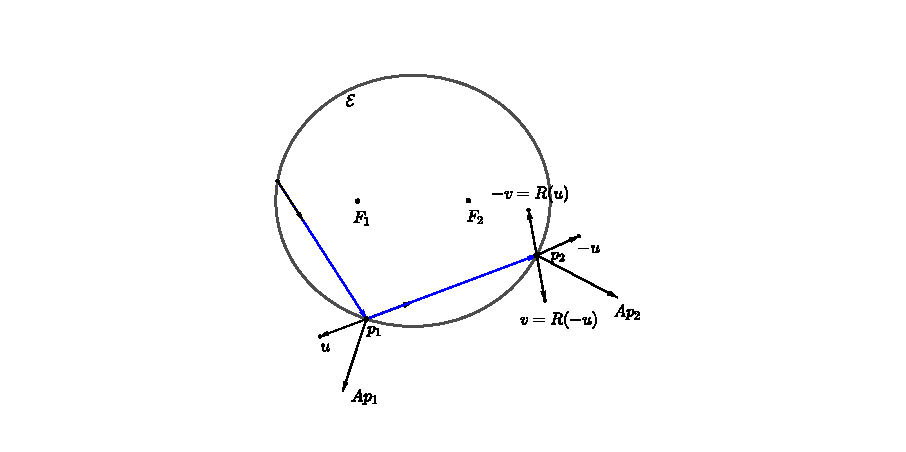
\includegraphics[trim=70 10 120 20,clip,width=\textwidth]{pics_tex/joachimstall.pdf}
	 %	 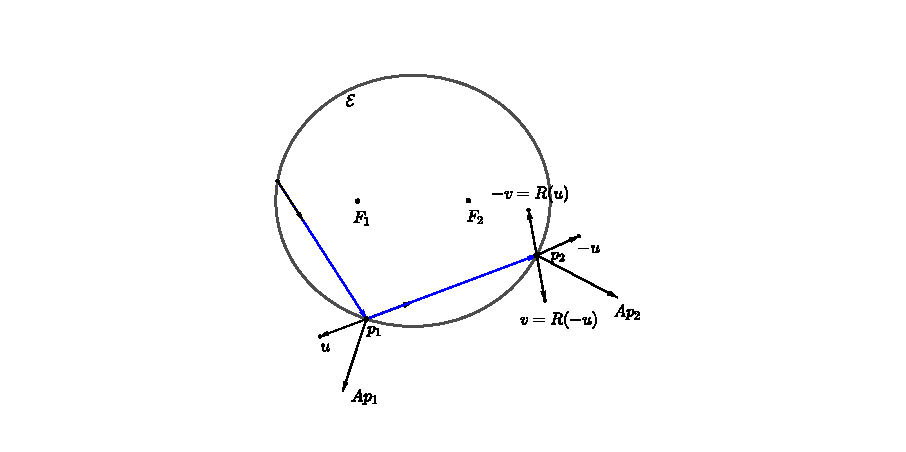
\includegraphics[scale=0.9]{pics_tex/joachimstall.pdf}
		\caption {Joachimsthal's first integral  $ \langle Ap_1,u\rangle $ is T-invariant.}
		 \label{fig:joachim}
	\end{center}
\end{figure}

\begin{proof} The tangent space  $T_{p}\mathcal{E}$ is formed of the vectors $u$ such that $ \langle Ap,u\rangle =0.$ Therefore $Ap$ is a normal vector to the ellipse at the point $p$. The vector $u$ is proportional to $p_2-p_1$.
	
	Therefore,
	\begin{align*}  \langle Ap_1+Ap_2 , p_2-p_1\rangle &= \langle Ap_1  , p_2 \rangle + \langle Ap_2  , p_1 \rangle  - \langle Ap_1  , p_1 \rangle + \langle Ap_2  , p_2 \rangle \\
	&= \langle  p_1  , Ap_2 \rangle - \langle Ap_2  , p_1 \rangle =0. 
	\end{align*}
	Then,
	\[ \langle Ap_1 , u\rangle =\langle  Ap_2 ,-u\rangle  =  \langle  Ap_2 ,R(-u)\rangle  =  \langle  Ap_2, v\rangle \]
	\end{proof}